%!TEX root = Slic3r-Manual.tex

\section{Combatre le Suintement} % (fold)
\label{sec:fighting_ooze}
\index{ooze}
\index{suintement}
\index{retraction}
\index{retractation}


\`a moins que le mat\'eriau en cours d'extrusion ait une viscosit\'e tr\`es \'elev\'ee, il va suinter de la buse entre les deux extrusions. Il ya plusieurs param\`etres dans Slic3r qui peuvent aider \`a y rem\'edier.

Les param\`etre de retractation, de l'onglet \texttt{Printer} (Imprimante),indiquer \`a l'imprimante de retirer le filament entre les mouvements d'extrusion. Cela peut r\'eduire la pression dans la buse, ce qui r\'eduit suintement. Apr\`es un d\'eplacement, la r\'etractation est invers\'e pour pr\'eparer l'extrudeuse pour la prochaine extrusion.

\begin{figure}[H]
\centering
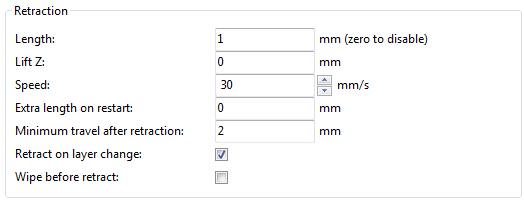
\includegraphics[keepaspectratio=true,width=1.0\textwidth]{expertmode/retraction_settings.png}
\caption{Param\`etres de retractation.}
\label{fig:retraction_settings}
\end{figure}
\index{Printer Settings!Extruder!Retraction!Length}
\index{Param\`etre de l'Imprimante!Extrudeuse!R\'etractation!Longueur}
\index{Printer Settings!Extruder!Retraction!Lift Z}
\index{Param\`etre de l'Imprimante!Extrudeuse!R\'etractation!Lever Z}
\index{Printer Settings!Extruder!Retraction!Speed}
\index{Param\`etre de l'Imprimante!Extrudeuse!R\'etractation!Vitesse}
\index{Printer Settings!Extruder!Retraction!Extra length on restart}
\index{Param\`etre de l'Imprimante!Extrudeuse!R\'etractation!Longueur suppl\'ementaire au red\'emarrage}
\index{Printer Settings!Extruder!Retraction!Minimum travel after retraction}
\index{Param\`etre de l'Imprimante!Extrudeuse!R\'etractation!D\'eplacement minimum apr\`es r\'etractation}
\index{Printer Settings!Extruder!Retraction!Retract on layer change}
\index{Param\`etre de l'Imprimante!Extrudeuse!R\'etractation!R\'etractation au changement de couche}
\index{Printer Settings!Extruder!Retraction!Wipe before retract}
\index{Param\`etre de l'Imprimante!Extrudeuse!R\'etractation!Essuyer avant r\'etractation}

\begin{itemize}
    \item \texttt{Length} (Longueur) - Le nombre de millim\`etres \`a r\'etracter. A noter que la mesure est effectu\'ee \`a partir du filament brut entrant dans l'extrudeuse. Une valeur comprise entre 1 et 2 mm est habituellement recommand\'e. Extrudeuses d\'eport\'ee peuvent avoir besoin de 4 ou 5 mm en raison de l'hyst\'er\'esis introduit par le tube.
    \item \texttt{Lift Z} (Lever Z) - Soul\`eve l' extrudeuse sur l'axe Z de quelque millim\`etres pendant chaque d\'eplacement. Cela peut \^etre utile pour s'assurer que la buse n'accroche pas un filament d\'ej\`a d\'epos\'e, mais ceci n'est g\'en\'eralement pas n\'ecessaire et ralentit la vitesse d'impression. Une valeur de 0,1 mm est g\'en\'eralement suffisante.
    \item \texttt{Speed} (Vitesse) - La vitesse \`a laquelle le moteur de l'extrudeuse va retirer le filament. La valeur doit \^etre d\'efinie \`a une vitesse que l'extrudeuse peut g\'erer sans sauter des pas, et il est int\'eressant d'exp\'erimenter plusieurs valeurs pour trouver le retrait le plus rapide possible.
    \item \texttt{Extra length on restart} (Longueur suppl\'ementaire au red\'emarrage) -  Ajoute une longueur suppl\'ementaire de fil apr\`es que le retrait soit compens\'e \`a la fin du d\'eplacement. Ce param\`etre est rarement utilis\'e, mais il le doit, si l'impression montrent des signes de manque de mati\`ere apr\`es la fin du d\'eplacement, alors il peut \^etre utile d'ajouter une petite quantit\'e de mati\`ere suppl\'ementaire.
    \item \texttt{Minimum travel after retraction} (D\'eplacement minimum apr\`es r\'etractation) - D\'eclenchement d'une r\'etractation apr\`es des mouvements tr\`es courts est g\'en\'eralement inutile, car la quantit\'e de suintement est g\'en\'eralement n\'egligeable et il ralentit le temps d'impression.  D\'efinis le nombre de millim\`etres minimum que la buse peut parcourir avant d'envisager une r\'etractation.  Si l'imprimante g\'ere bien le suintement cette valeur peut \^etre augment\'ee \`a 5 ou 6 mm.
    \item \texttt{Retract on layer change} (R\'etractation au changement de couche) - Le mouvement le long de l'axe Z, doit \'egalement \^etre consid\'er\'e lorsqu'il s'agit du suintement, sinon des gouttes peuvent se produire. Il est recommand\'e de laisser ce param\`etre coch\'e.
    \item \texttt{Wipe before retract} (Essuyer avant r\'etractation) - D\'eplace la buse tout en r\'etractant de mani\`ere \`a r\'eduire les risques de formation d'une goutte.
\end{itemize}


En outre, il ya plusieurs param\`etres dans l'onglet \texttt{Print Settings} (Param\`ete de l'Imprimante) qui peuvent aider \`a contr\^oler le suintement.

\begin{itemize}
    \index{Print Settings!Infill!Advanced!Only retract when crossing perimeters}
	\index{Param\`etres d'Impression!Remplissage!Advanc\'e!Retrait seulement lors du croisement avec uns p\'erim\`etre}
    \item \texttt{Only retract when crossing perimeters} , Retrait seulement lors du croisement avec uns p\'erim\`etre (Infill - Advanced) (Remplissage - Avanc\'e) - Indique \`a Slic3r de ne r\'etracter que si la buse traverse le bord de l'\^ile qui vient d' \^etre extrud\'ee. De l\'eger suintement dans les murs d'une pi\`ece ne sont pas perçus et peuvent g\'en\'eralement \^etre accept\'ee.
    \index{Print Settings!Layers and perimeters!Quality!Avoid crossing perimeters}
    \index{Param\`etres d'Impression!Couches et p\'erim\`etres!Qualit\'e!Evitez de croiser les p\'erim\`etres}
	\item \texttt{Avoid crossing perimeters} , Evitez de croiser les p\'erim\`etres (Layers and perimeters - Quality) (Couches et p\'erim\`etres - Qualit\'e) - Forcera la buse \`a suivre les p\'erim\`etres autant que possible afin de minimiser le nombre de fois o\`u il doit les traverser en se d\'eplaçant, et entre les \^iles. Cela a un impact n\'egatif \`a la fois sur la g\'en\'eration G-code et le temps d'impression.
    \index{Print Settings!Layers and perimeters!Advanced!Randomize starting points}
    \index{Param\`etres d'Impression!Couches et p\'erim\`etres!Avanc\'e!Points de d\'epart al\'eatoire}
	\item \texttt{Randomize starting points} , Points de d\'epart al\'eatoire (Layers and perimeters - Advanced) (Couches et p\'erim\`etre - Avanc\'e) - Comme l'extrudeuse se d\'eplace vers le haut pour le d\'ebut de la couche suivante, tout suintement peut entra\^iner des des gouttes. Si le m\^eme point de d\'epart est utilis\'ee pour chaque couche puis une couture peut se former le long de l'objet. Ce r\'eglage d\'eplacera le point de d\'epart \`a un emplacement diff\'erent pour chaque couche.
\end{itemize}


Voir aussi la section \ref{par:sequential_printing}: Impression S\'equentielle, pour une autre technique qui peut minimiser ficelles se formant entre les objets.
% section fighting_ooze (end)